\documentclass[12pt]{article}

\usepackage{epsfig,a4wide,amsmath,amssymb,amsfonts,mathrsfs}
\usepackage{ulem}

\usepackage[colorlinks=true]{hyperref}
\usepackage{enumitem}

\pagestyle{headings}

\newcommand{\du}{\mathrm{d}}

 \setlength{\abovecaptionskip}{1ex}
 \setlength{\belowcaptionskip}{1ex}
 \setlength{\floatsep}{1ex}
 \setlength{\textfloatsep}{1ex}

% \setlength{\textwidth}{17cm}
% \setlength{\oddsidemargin}{-0.4cm}
% \setlength{\topmargin}{0.0cm}
% \setlength{\textheight}{22cm}
% \setlength{\parindent}{0.5cm}

\numberwithin{equation}{section}

\renewcommand{\textfraction}{0}
\renewcommand{\topfraction}{1}
\renewcommand{\floatpagefraction}{1}

\newcommand*{\defeq}{\mathrel{\vcenter{\baselineskip0.5ex \lineskiplimit0pt
                     \hbox{\scriptsize.}\hbox{\scriptsize.}}}%
                     =}
\newcommand*{\invdefeq}{=\mathrel{\vcenter{\baselineskip0.5ex \lineskiplimit0pt
                     \hbox{\scriptsize.}\hbox{\scriptsize.}}}%
                     }
\newcounter{count}

\normalem

\title{Notes on boson stars in scalar-tensor theory and code infrastructure}
\author{Tamara Evstafyeva}
\date{}
\begin{document}
\maketitle
% \tableofcontents
\newpage

%=============================================================================
\section{Theory action}
In the Einstein frame
\begin{equation}
  S_E = \frac{1}{16\pi G} \int \du x^4 \sqrt{-\bar{g}}
  \left\{
  \bar{R}-2\bar{g}^{\mu\nu} \partial_{\mu} \varphi\,
  \partial_{\nu}\varphi-4W(\varphi)
  \right\}
  %+ S_m [\psi_m,a^2(\varphi) \bar{g}_{\mu\nu}]\,,
  + S_m [\psi_m,F(\varphi)^{-1} \bar{g}_{\mu\nu}]\,.
  \label{eq:SE}
\end{equation}
In the Jordan, aka physical, frame
\begin{equation}
  S_J = \int \du x^4 \sqrt{-g} \left\{
  \frac{F(\phi)}{16\pi G} R
  - \frac{1}{2} g^{\mu\nu}\partial_{\mu}\phi\,\partial_{\nu}\phi
  - U(\phi)
  \right\}
  +
  S_m(\psi_m,g_{\mu\nu})\,,
  \label{eq:SJ}
\end{equation}
where in the physical frame the matter counterpart is given via a bosonic action
\begin{equation}
  S_m = \int \du x^4 \sqrt{-g} \left\{
  -\frac{1}{2} \left[ g^{\mu\nu}\nabla_{\mu}\psi^*\,\nabla_{\nu} \psi
  + V(\psi)\right]\,
  \right\}.
\end{equation}

%=============================================================================
\section{Variables}
To avoid confusion, I have mainly used the variables of Uli's notes, i.e.
\begin{itemize}
    \item $A$ -- amplitude of the bosonic scalar field.
    \item $\omega$ -- frequency of the boson star, in the code we start with initial guess of $\omega =1$, but this can be changed if searching for other solutions.
    \item $\varphi$ -- gravitational scalar field.
    \item $\alpha$ -- lapse function.
    \item $X$ -- function of $r$ from line-element ansatz $\du s^2 = -\alpha^2 \du t^2 + X^2 \du r^2 + \frac{r^2}{F} \du \Omega^2$.
    \item $W(\varphi)$ -- potential function for the gravitational scalar field given by $W(\varphi) = \frac{1}{2}\mu_{\varphi}^2 \varphi^2$, where $\mu_{\varphi}^2$ is the mass variable.
    \item $V(A^2)$ -- solitonic potential for the bosonic scalar field defined by $V(A^2) = A^2\left(1 - 2\frac{A^2}{\sigma_0^2}\right)^2$.
    \item $F(\varphi)$ -- conformal factor defined by $F(\varphi) = e^{-2\alpha_0 \varphi-\beta_0\varphi^2}$.
\end{itemize}
To have only first order derivatives, we further introduce the following auxiliary variables
\begin{align}
    \partial_r \varphi &= X \eta, \\
    \partial_r A &= \Psi_0.
\end{align}
We also choose to use $\Phi$ instead of the lapse $\alpha$, which is defined as
\begin{equation}
    \Phi = \rm{ln} \left(\sqrt{F} \alpha \right).
\end{equation}
Finally, we note that
\begin{equation}
    \frac{\partial_r F}{F} = \frac{F_{, \varphi}}{F}\partial_r \varphi = \frac{F_{, \varphi}}{F}X \eta.
\end{equation}


%=============================================================================
\section{Equations of integration}
Below we detail the equations that we implement for outward integration in the code. Note that the set of variables we are solving for is given by $\{\Phi, X, \eta, \Psi_0 \}$.
\begin{eqnarray}
  \partial_r \Phi
  &=&
  \frac{FX^2-1}{2r}
  -rFX^2W
  +\frac{r}{2}(X \eta)^2
  +2\pi r\frac{X^2}{F}\left[
  \frac{\Psi_0^2}{X^2}
  +\frac{A^2 \omega^2}{\alpha^2}
  -V
  \right]\,,
  \label{eq:Phir}
  \\[10pt]
  \frac{\partial_r X}{X}
  &=&
  -\frac{FX^2-1}{2r}
  +rFX^2W
  -\frac{1}{2}\frac{F_{, \varphi}}{F} X \eta
  +\frac{r}{2}(X \eta)^2
  +2\pi r\frac{X^2}{F}
  \left[
  \frac{\Psi_0^2}{X^2}
  +\frac{A^2 \omega^2}{\alpha^2}
  +V
  \right]\,,
  \label{eq:Xr}
  \\[10pt]
  \partial_r \eta
  &=&
  -\eta \left(
  \partial_r \Phi
  -\frac{1}{2} \frac{F_{, \varphi}}{F} X \eta
  \right)
  -\frac{2}{r}\eta
  + FX^2 W_{,\varphi}
  +\frac{2\pi XF_{,\varphi}}{F^2}
  \left[
  \frac{A^2\omega^2}{\alpha^2}
  -\frac{\Psi_0^2}{X^2}
  -2V
  \right]\,,
  \label{eq:etar}
  \\[10pt]
  \partial_r \Psi_0 &=&
  -2\frac{\Psi_0}{r}
  +\Psi_0 \left(
  \frac{\partial_r X}{X}
  + \frac{3}{2}\frac{\partial_r F}{F}
  - \partial_r \Phi
  \right)
  - \frac{X^2\omega^2 A}{\alpha^2}
  + X^2V_{\,,|\psi|^2} A\,,
%  - \frac{X^2\omega^2 \textcolor{red}{A} \cancel{A^2}}{\alpha^2}
%  + \textcolor{red}{X^2V_{\,,|\psi|^2} A}\cancel{X^2V_{\,|\varphi|^2} A}\,.
  \label{eq:Psi0r}
\end{eqnarray}
where I was lazy to replace $\alpha \rightarrow e^{\Phi}/\sqrt{F}$.

%=============================================================================
\section{Boundary conditions at the origin}
At $r = 0$, the boundary condition are
\begin{align}
    &\partial_r \varphi (r = 0) = 0 \implies \eta(r = 0) = 0, \\
    &\partial_r A (r = 0) = 0, \\
    &\Phi(r = 0) = 1, \\
    &A(r = 0) = A_{\rm{c}} \quad \text{(user-specified)}, \\
    &X(r = 0) = \frac{1}{\sqrt{F(\varphi(0))}}, \\
    &\varphi(r = 0) = \varphi_{\rm{c}} \quad \text{(user-specified but is checked and improved until surface condition is satisfied)}.
    \label{eq:bcsattheorigin}
\end{align}

%=============================================================================
\section{Series expansion near the origin}
Using the boundary condition at the origin \eqref{eq:bcsattheorigin}, we are able to derive the behaviour of our PDEs at the origin, which in the code are implemented within an open ball of small radius ($r_{\rm{small}} = 10^{-15}$)
\begin{align}
    \partial_r \Phi &= 0, \\
    \partial_r X & = 0, \\
    \partial_r \Psi_0 &= \frac{1}{3} \left(\frac{1}{F} V_{\,,|\psi|^2} A - \omega^2 A e^{-2 \Phi} \right), \\
    \partial_r \eta & = \frac{1}{3} \left[\sqrt{F({\varphi(0))}} W_{, \varphi} + \frac{2 \pi F_{, \varphi}}{F^2 \sqrt{F}}
     \left(\frac{\omega^2 A^2 F}{e^{2 \Phi}} - 2V \right) \right].
\end{align}

%=============================================================================
\section{Conversion to isotropic radius}
If one prefers to work with isotropic radius, here we present how their radial quantities are related. This is also coded up in the $1D$-solver. I'd expect the isotropic line-element ansatz for the scalar-tensor theory would take the following form
\begin{equation} \label{eq:iso_line}
    {\rm d}s^2 = -F \alpha^2 {\rm d}t^2 + F \psi^4 \left({\rm d}R^2 +R^2 {\rm d}\Omega^2 \right).
\end{equation}
Comparing it with the areal-radius line-element, which is assumed to be
\begin{equation} \label{eq:areal_line}
    {\rm d}s^2 = -F \alpha^2 {\rm d}t^2 + F X^2 {\rm d}r^2 +r^2 {\rm d}\Omega^2,
\end{equation}
we find the following relations between the variables
\begin{equation}
    F \psi^4 R^2 = r^2 \quad \text{ and } \quad  \psi^4 {\rm d}R^2 = X^2 {\rm d}r^2.
\end{equation}
The latter equation has a singular nature, making our lives harder, so in order not to deal with singularities, we introduce a new variable
\begin{equation} \label{eq:f-func}
    f(r) \defeq \frac{R}{r} \quad \implies \quad \frac{{\rm d}f}{{\rm d}r} = \frac{f}{r}\left(X\sqrt{F}-1\right).
\end{equation}
At the origin, we know that $X(r = 0) = 1/\sqrt{F(\varphi(0))} + \mathcal{O}(r^2)$ and so in the derivative equation for $f(r)$, \eqref{eq:f-func}, the bracket becomes zero and the radii relate linearly, in other words $R \propto r$. In the code, we therefore set $f=1$ initially and integrate it out; after that we re-scale it appropriately by requiring that both radii agree at infinity. We can do this, since any kind of multiplication of the solution by a constant still gives us the solution to the ODE.

Now, to find this appropriate re-scaling to the $f(r)$ solution, we equate the areas resulted from the line-elements \eqref{eq:iso_line}--\eqref{eq:areal_line} and for large radii approximate the conformal factor of the isotropic line-element via $\psi = 1 - m/(2R)$. By doing so the equality simplifies to the following
\begin{equation}
    r^2 = F \left(1- \frac{m}{2R} \right)^4 R^2.
\end{equation}
After some algebraic manipulations, we then obtain the following radial relations
\begin{equation}
    R = \left(\frac{r}{\sqrt{F}} -m \right) - \frac{1}{4}\frac{\sqrt{F}m^2}{\left(r - \sqrt{F}m \right)} \quad \Leftrightarrow \quad r = \sqrt{F} \left(m + R + \frac{1}{4}\frac{m^2}{R} \right),
\end{equation}
which reduce to the GR case in the limit, $F \to 1$ (see Uli's notes on BSs).

%=============================================================================
\section{Asymptotic behaviour}
Whilst the asymptotics turned quite out tricky and we have identified 3 cases that should be analysed separately for when $\alpha_0 \neq 0$ (with 2 of them being 'physical'). We focus on the case when $h < 2k$, which forces most of the 'nasty' terms to cancel in the asymptotic behaviour of the equations. This means the asymptotic behaviours of the bosonic scalar field and the gravitational scalar field are summarized as follows
\begin{align}
    \varphi & \sim \frac{e^{-hr}}{r^{1+\delta}}, \quad \text{where} \quad h=m \quad \text{and} \quad \delta = Mm = Mh, \label{eq:gravitational_asym}  \\
    A & \sim \frac{e^{-kr}}{r^{1+\epsilon}}, \quad \text{where} \quad k=\sqrt{1-\omega^2} \quad \text{and} \quad \epsilon = M\frac{1-2\omega^2}{k} = M\frac{2k^2-1}{k}, \label{eq:boson_asym} 
\end{align}
where we estimate the mass $M$ using the mass function $m(r) \defeq \frac{r}{2} \left(1-\frac{1}{FX^2}\right)$ and the frequency $\omega$ through the shooting algorithm. It is crucial to note that we also need to reinforce that the lapse function goes to unity at infinity, that is $\lim_{r \to \infty} \alpha = 1$. We can re-scale $\alpha$ (or $\Phi$ in our case), as long as we re-scale $\omega$ with it! This is achieved via $\omega \rightarrow \omega e^{-\rm{ln}(\sqrt{F}X) -\rm{ln}(\sqrt{F}\alpha)}$.

%=============================================================================
\section{Methodology for the massless case}
The idea is pretty much the same as for our 'classic' boson stars. Briefly, this means that we take our equations \eqref{eq:Phir}--\eqref{eq:Psi0r} and integrate them outwards until some $r_{stop}$, where the solution for the bosonic field diverges and goes bonkers. From $r_{stop}$ we set the bosonic variable counterparts to zero to avoid crashing the code. We then find the minimum of the bosonic scalar field before it starts to diverge, and glue the asymptotic behavior to it. 

We concentrate on the \textit{massless} case for the time being, and in this case we do not use the asymptotic behavior for $\varphi$, as it is super slow, but rather just continue integrating outwards the equation for the gravitational scalar field. We repeat the whole integration from the point of asymptotic matching, now hopefully getting a physical solution. 

Usually any initial guess for $\varphi_{\rm{c}}$ produces something. However, is it what we are looking for? Sadly, not really. To enforce 'the correct solution' in the code, we use the surface condition equation for the gravitational scalar field by Damour \cite{Damour:1993hw, Gerosa:2016fri}. It is in principle applicable to vacuum, however far away (at large radius) the boson star is fairly 'vacuum', we assume it is an alright for us approximation to use. The condition gives the expected value for the gravitational scalar field on the surface of the star, or just 'far enough' for our case
\begin{equation} \label{eq:Damour_condition}
    \varphi_{\rm{s}} = - \frac{X_{\rm{s}} \eta_{\rm{s}}}{\sqrt{(\partial_r \Phi_{\rm{s}})^2 + X_{\rm{s}} \eta_{\rm{s}}}} \rm{artanh} \frac{\sqrt{(\partial_r \Phi_{\rm{s}})^2 + X_{\rm{s}} \eta_{\rm{s}}}}{\partial_r \Phi_{\rm{s}} + 1/r_{\rm{s}}}.
\end{equation}
Here by 's' we denote the variable evaluated on the star's surface. In our code the surface is defined as just a few gridpoints away from the edge of the grid. We quantity how well this condition is satisfied by comparing it with our numerical value for $\varphi$ at that surface point, and improve on the central field guess $\varphi_{\rm{c}}$ until we meet this surface condition up to some satisfactory tolerance (i.e. $10^{-5}$) using Newton-Raphson algorithm.

\section{$\alpha_0 = 0$ case}
Here we explore what happens when we have $\alpha_0 = 0$ fixed. Let us consider here a rather extremely negative choice for $\beta_0$, such as $\beta_0 = -12$. We find two solutions giving symmetric profiles for the gravitational scalar field, $\varphi$, across the horizontal axis, which correspond to the positive and negative solutions for $\varphi$. They also produce an additional branch of solutions on the $M(R)$ plot in Fig.~\ref{fig:alpha00}. The feature of these 'mirror' solutions is very much as in the neutron star case \cite{Rosca-Mead:2020bzt}. When $\varphi_{\rm c} = 0$, as expected, we recover exactly the GR solution for the bosonic scalar field. The reason for such a negative value of $\beta_0$ chosen here is that for $\beta_0 \leq -8$ (which was obtained roughly empirically), the central values for the gravitational field are of at most $\mathcal{O}(10^{-5})$ and therefore not very much interesting.

\begin{figure}
    \centering
    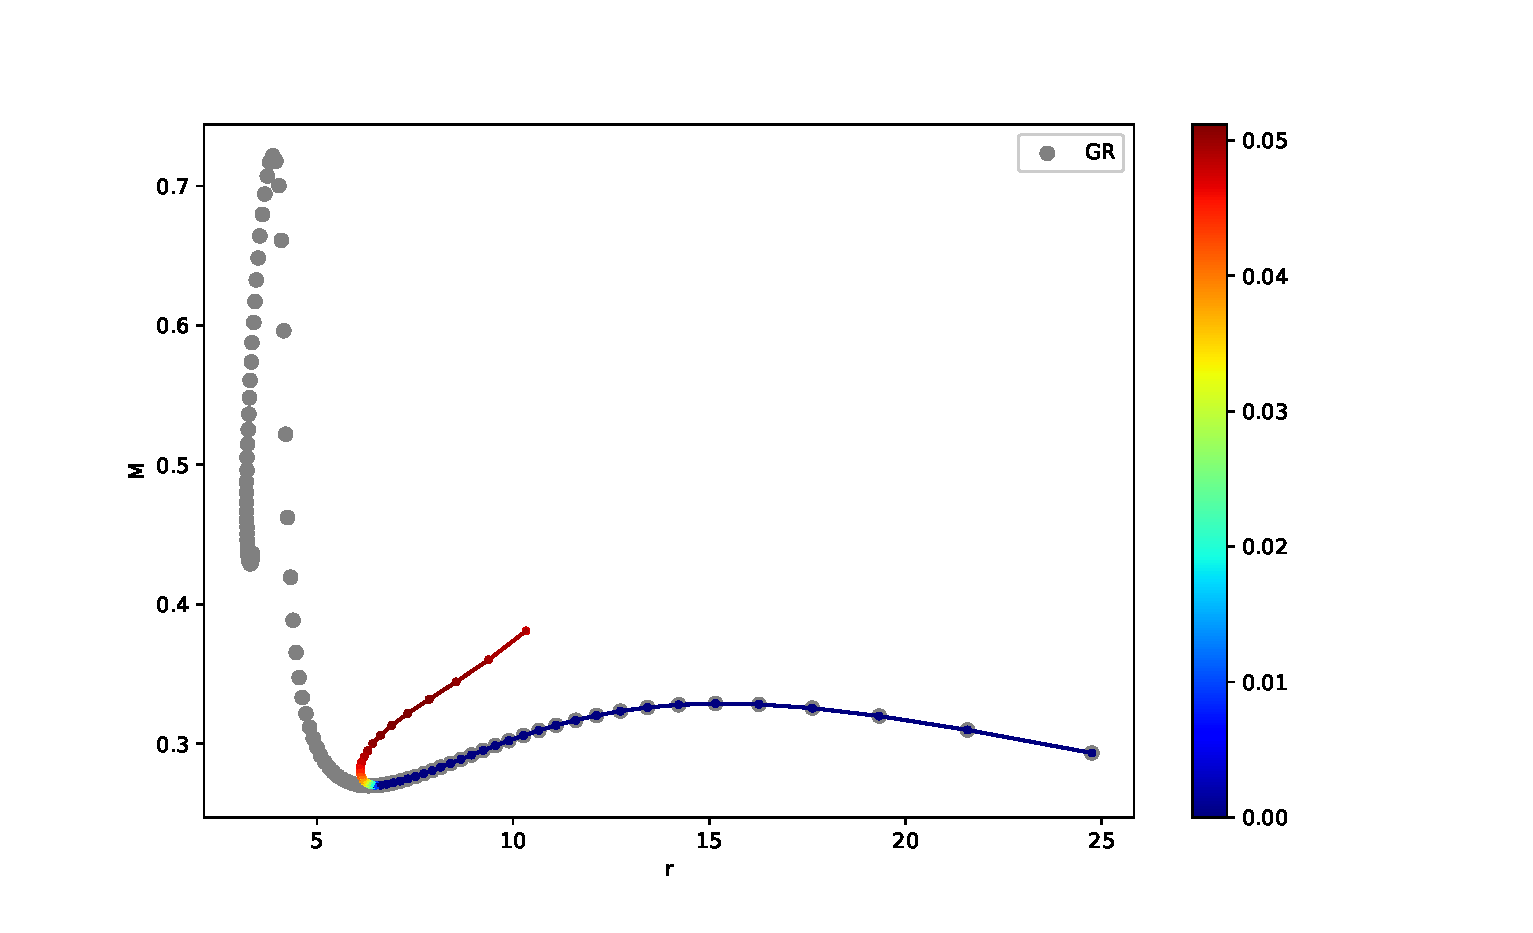
\includegraphics[width=0.8\textwidth, clip=True]{massles_beta12_alpha0.eps}
    \caption{Boson star central amplitude in GR and ST theory. Here we set $\beta_0 = -12$, for which am additional branch of solutions appears.}
    \label{fig:alpha00}
\end{figure}

\section{Dependence on $\alpha_0$} 
\label{sec:massless_sols_alpha0}
In this section, we investigate the effect of changing $\alpha_0$, whilst keeping $\beta = -4.5, A_{\rm c} = 0.147$ fixed (which is roughly around the most negative value allowed by the constraints). Figure \ref{fig:alpha_var} demonstrates the family of solutions for this case. In particular, we see that small values of $\alpha_0 \leq 0.01$ result in solutions not very much different from the GR ones. However, as we start to increase the value of $\alpha_0$, another branch of solutions starts to appear, by tilting to the right, away from the GR branch. The additional branch of solutions however still represents the weakly scalarised solutions.
\begin{figure}
    \centering
    \includegraphics[width=0.45\textwidth, clip=True]{MofR_alpha001.eps} 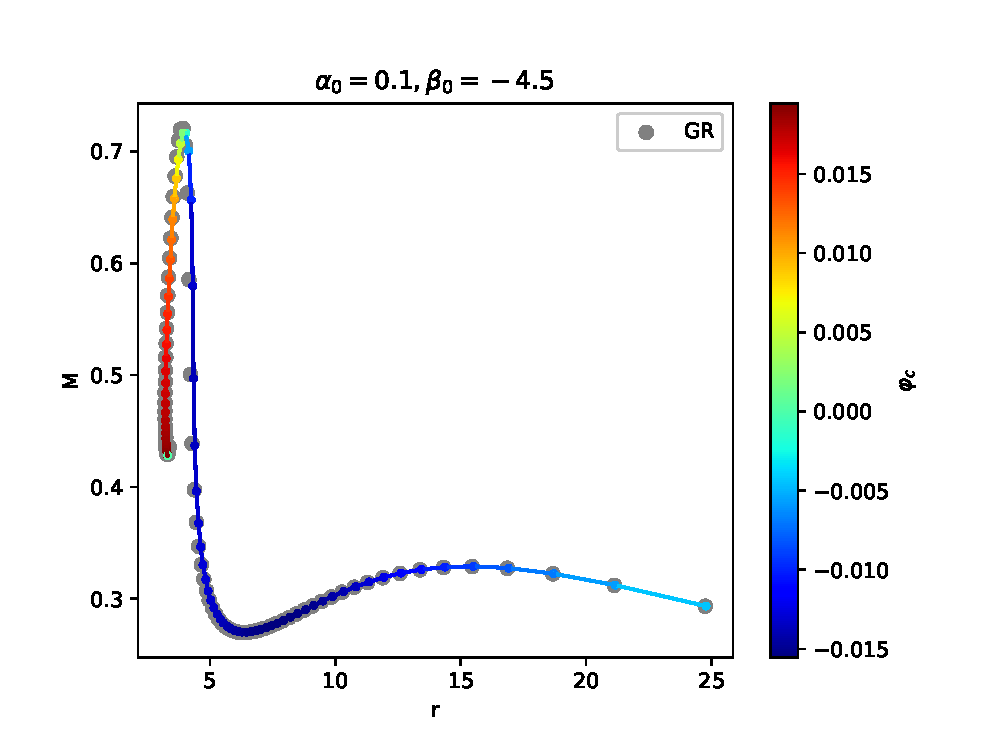
\includegraphics[width=0.45\textwidth, clip=True]{MofR_alpha01.eps} \\
    \includegraphics[width=0.45\textwidth, clip=True]{MofR_alpha03.eps} \includegraphics[width=0.45\textwidth, clip=True]{MofR_alpha05.eps} \\
    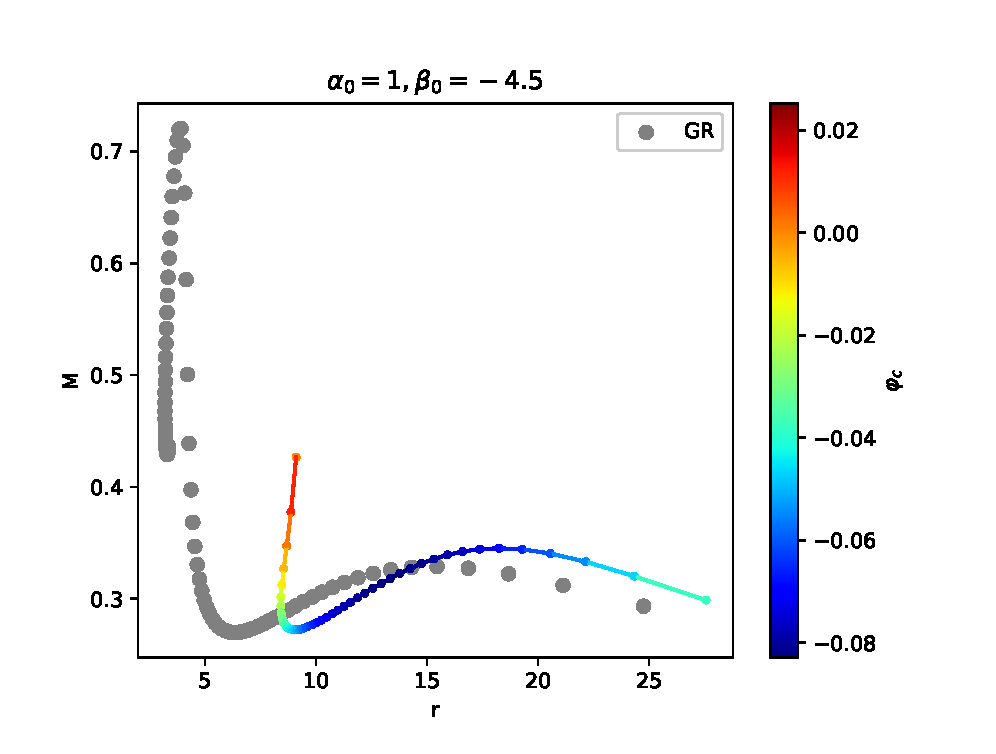
\includegraphics[width=0.45\textwidth, clip=True]{MofR_alpha1.eps}
    \caption{Dependence of solutions on the varying $\alpha_0$ and fixed $\beta_0 = -4.5, A_{\rm c} = 0.147$. The grey circles represent GR solutions. As we increase $\alpha_0$, we find that the solution branch shifts away from the GR one and for very large values 'breaks down', no longer representing a certain range of $M(R)$ plot.}
    \label{fig:alpha_var}
\end{figure}

\section{Dependence on $\beta_0$} \label{sec:massless_sols_beta0}
It seems to be easier to find strongly scalarised solutions, $|\varphi_{\rm c}| \sim \mathcal{O}(\alpha_0)$, when varying $\beta_0$. Typically, with \textit{very} negative values of $\beta_0$, e.g. $\beta_0 = -12.0$, we can find such strongly scalarised solutions. As an example for illustration purposes, let us choose $\beta_0 = -12$, $\alpha_0 = 0.01$ and $A_{\rm{c}} = 0.147$. In this case, as illustrated in Fig.~\ref{model-beta-12}, it is possible to recover weakly and strongly scalarised solutions, depending on the central guess for the gravitational scalar field.

\begin{figure}
    \centering
    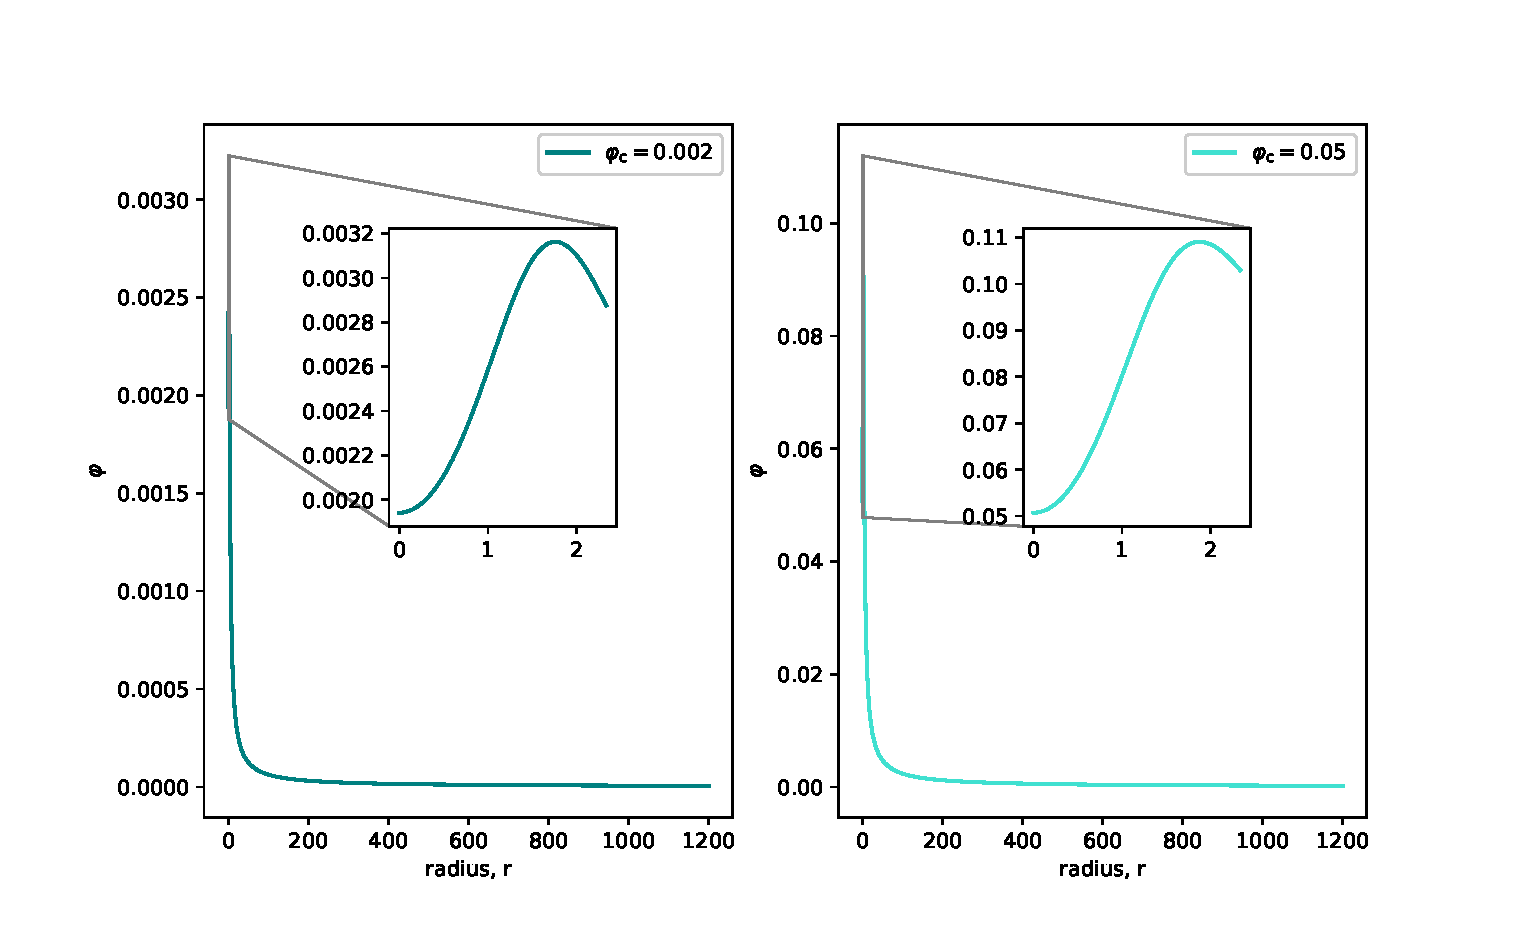
\includegraphics[width=15cm]{model-beta-12.eps}
    \caption{Profile of the gravitational scalar field as a function of the radius, computed from different initial guesses for $\varphi_{\rm{c}}$. One yields a profile of roughly $\mathcal{O}(\alpha)$, whereas the other one results in much more scalarisation giving $\varphi \sim \mathcal{O}(1)$; the asymptotic condition is satisfied for both cases.}
    \label{model-beta-12}
\end{figure}

Further, by varying the central amplitude of the bosonic field, $A_{\rm{c}}$, we construct $M(R)$ of plot in Fig.~\ref{fig:MofR_betavar}. In general, smaller values of $\beta_0$ give $M(R)$ curves closer to the GR case, as expected. For example, in the case of $\beta_0 = -6$, the branch with additional solutions lies close to the GR branch, but ever slightly deviates and reaches the values of $|\varphi_{\rm c}|$ corresponding to strongly scalarised case. As we increase $\beta_0$ in magnitude (whilst still keeping it negative), the branch shrinks and tilts to the right (in the similar way as for when we varied the values of $\alpha_0$ parameter). The key difference for much larger values of $\beta_0$ is that we now also acquire strongly scalarised solutions with positive central value for the gravitational scalar field.

\begin{figure}
    \centering
    \includegraphics[width=0.45\textwidth, clip=True]{MofR_beta6.eps} 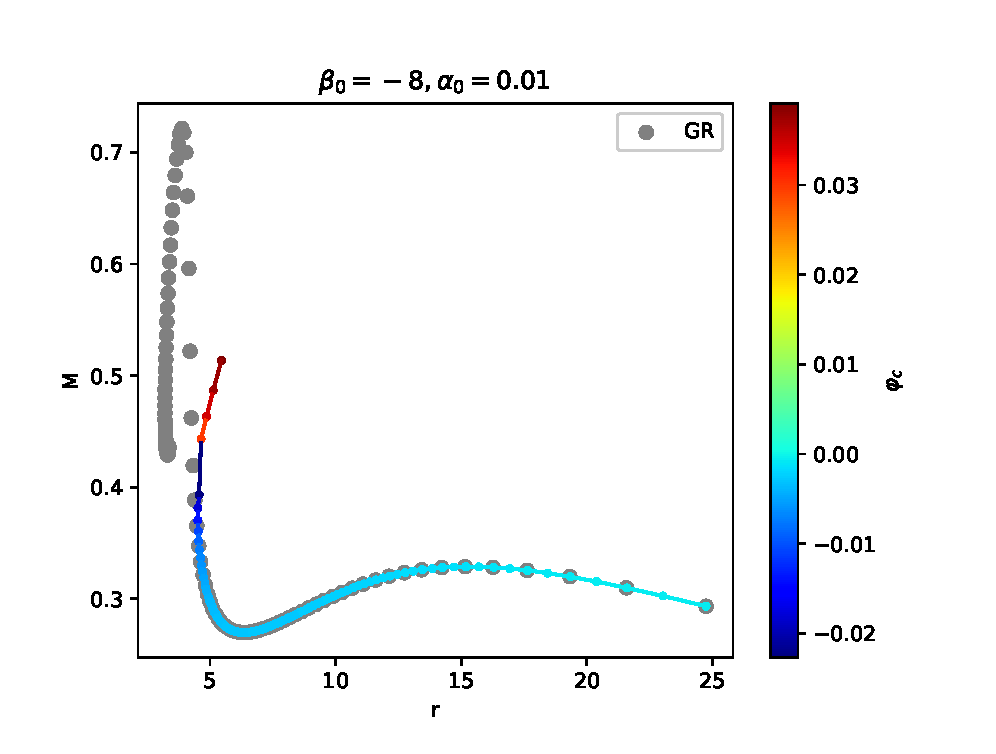
\includegraphics[width=0.45\textwidth, clip=True]{MofR_beta8.eps} \\
    \includegraphics[width=0.45\textwidth, clip=True]{MofR_beta10.eps} \includegraphics[width=0.45\textwidth, clip=True]{MofR_beta12.eps} \\
    \caption{Dependence of solutions on the varying $\beta_0$ and fixed $\alpha_0 = -0.01, A_{\rm c} = 0.147$. The grey circles represent GR solutions. As we increase $\beta_0$ to more negative choices, we find that the branch disjoints itself from the GR one, entering the strongly scalarised regime.}
    \label{fig:MofR_betavar}
\end{figure}

%=============================================================================
\section{Methodology for the massive case} \label{sec:massive_methodology}
The way the code works for the massive code is a little different, and it is in fact a 'separate' one. The equations and assumed asymptotic behaviour are all the same, except for 2 main principle features.
\begin{enumerate}
    \item Both scalar fields now are matched to their corresponding asymptotic behaviours as in Eqs.~\eqref{eq:boson_asym}--\eqref{eq:gravitational_asym}. This matching to asymptotics happens in the following way. We find the diverging behavior of the fields at some finite radius and then search backwards for the local minimum. We then take 90\% buffer region from the point of local minimum -- this consequently defines our matching radius $r_{\rm match}$. The points where bosonic scalar field and gravitational scalar fields have to be matched usually occur at different radii.
    \item The stopping criteria in the form of Eq.~\eqref{eq:Damour_condition} is now swapped for an alternative condition to ensure that the matching is smooth. This is inspired by how the massless case is handled via Eqs.~(3.40)-(3.41) of Ref.~\cite{Comer:1997ns}. We recall that asymptotically the gravitational field behaves like
    \begin{equation} \label{eq:criteria_massive}
        \varphi = B r^{-1 - \delta} e^{-m_{\varphi} r},
    \end{equation}
    where $B$ is some constant. Differentiating this expression, we obtain 
    \begin{equation} \label{eq:Bconstant}
    \varphi'(r) = B r^{-2 - \delta} e^{-m_{\varphi}r} \left(-1 - \delta - r m_{\varphi} \right),
    \end{equation}
    which gives us a readily available expression for what $B$ is
    \begin{equation}
        B = \frac{\varphi'(r)}{-1-\delta-rm_{\varphi}}r^{2+\delta}e^{m_{\varphi}r}.
    \end{equation}
    Now, the most common issue in the shooting when finding a suitable solution for the gravitational scalar field is that it falls off too fast. The radius of matching is too small and so when we glue the solution at that point to the asymptotics, the solution does not look smooth enough. By ensuring that Eq.~\eqref{eq:criteria_massive} is satisfied at the radius of matching $r_{\rm{matching}}$ to some user-specified threshold (e.g. $10^{-6}$), we hope that the solver converges to some solution. If the computed $\varphi(r_{\rm{matching}})$ is not the expected value, then we change the initial value of the gravitational scalar field $\varphi(0)$ and repeat the whole procedure until the threshold requirement is met. Once this criterion is reached, the matching looks smooth.
\end{enumerate}

\subsection{Zero-crossings of the gravitational scalar field}
We already know that $A$ has $n$ number of zero crossings, which is quantised by the respective oscillation frequencies $\omega_n$; furthermore, the number of zero-crossings is a non-decreasing function of frequency, $\omega$. Could there be a similar effect for the behavior of the gravitational scalar field, where its central value $\varphi_{\rm c}$ determines the number of crossings?

To explore such possibility, we shoot for the frequency of the boson star $\omega$ searching for the ground states. Once we find appropriate frequency, we integrate the governing equations without matching the fields' behaviours to their asymptotics. We do set the fields to zero at some fixed radius, when they start to diverge -- this produces spikes in profiles but the behavior before these spikes is valuable for understanding the nature of zero-crossings of the gravitational scalar field.

Using the condition for smooth matching of Section \ref{sec:massive_methodology} we find the central value of the gravitational scalar field that produces a smooth solution, which we also hope is the physical one. This profile is presented in blue in Fig.~\ref{zero-crossings}. We see that it falls of sufficiently slow (never crossing the $x$-axis) and reaches small positive values, but then at some larger radius ($r \sim 55$) starts to diverge. When we match this solution to its asymptotics, as expected, it then produces a smooth profile -- yay! Now, what happens as we depart away from this central value and how does it affect the zero-crossings? The results shown in Fig.~\ref{zero-crossings} suggest that similarly to the bosonic case, the number of zero crossings of the gravitational field increases or at least stays the same with increased central value $\varphi_{\rm c}$. To be more precise, I only found cases where the gravitational scalar field never crosses the $x$-axis or crosses them once! The desired, smooth solution (in blue) appears to be the only 'viable' choice for asymptotic matching. All other guesses for $\varphi_{\rm c}$ around it produce profiles that either have one zero-crossing or diverge from a small radius.

The role of the central amplitude for the gravitational scalar field is therefore not totally equivalent to the bosonic $\omega$ and the number of crossings for the gravitational field is limited to one at maximum.

\begin{figure}
    \centering
    \includegraphics[width=10cm]{zero_crossings.eps}
    \caption{Profile of the gravitational scalar field found by shooting for $\omega$ and integrating out the equations without any asymptotic matching. The fields are set to zero when their amplitudes become large, and this is where the profiles produce spikes, which suddenly drop to zero.}
    \label{zero-crossings}
\end{figure}

\section{Example profile: massive case}
We now present some solutions for the massive case. Similarly to \ref{sec:massless_sols_beta0} we set $A_{\rm c} = 0.147$, $\beta_0 = -12.0$, $\alpha = 0.01$ and see what happens... Here we choose $m_{\varphi} = 0.1$. As illustrated in Fig.~\ref{model-beta-12-massive}, we can find a solution.
\begin{figure}
    \centering
    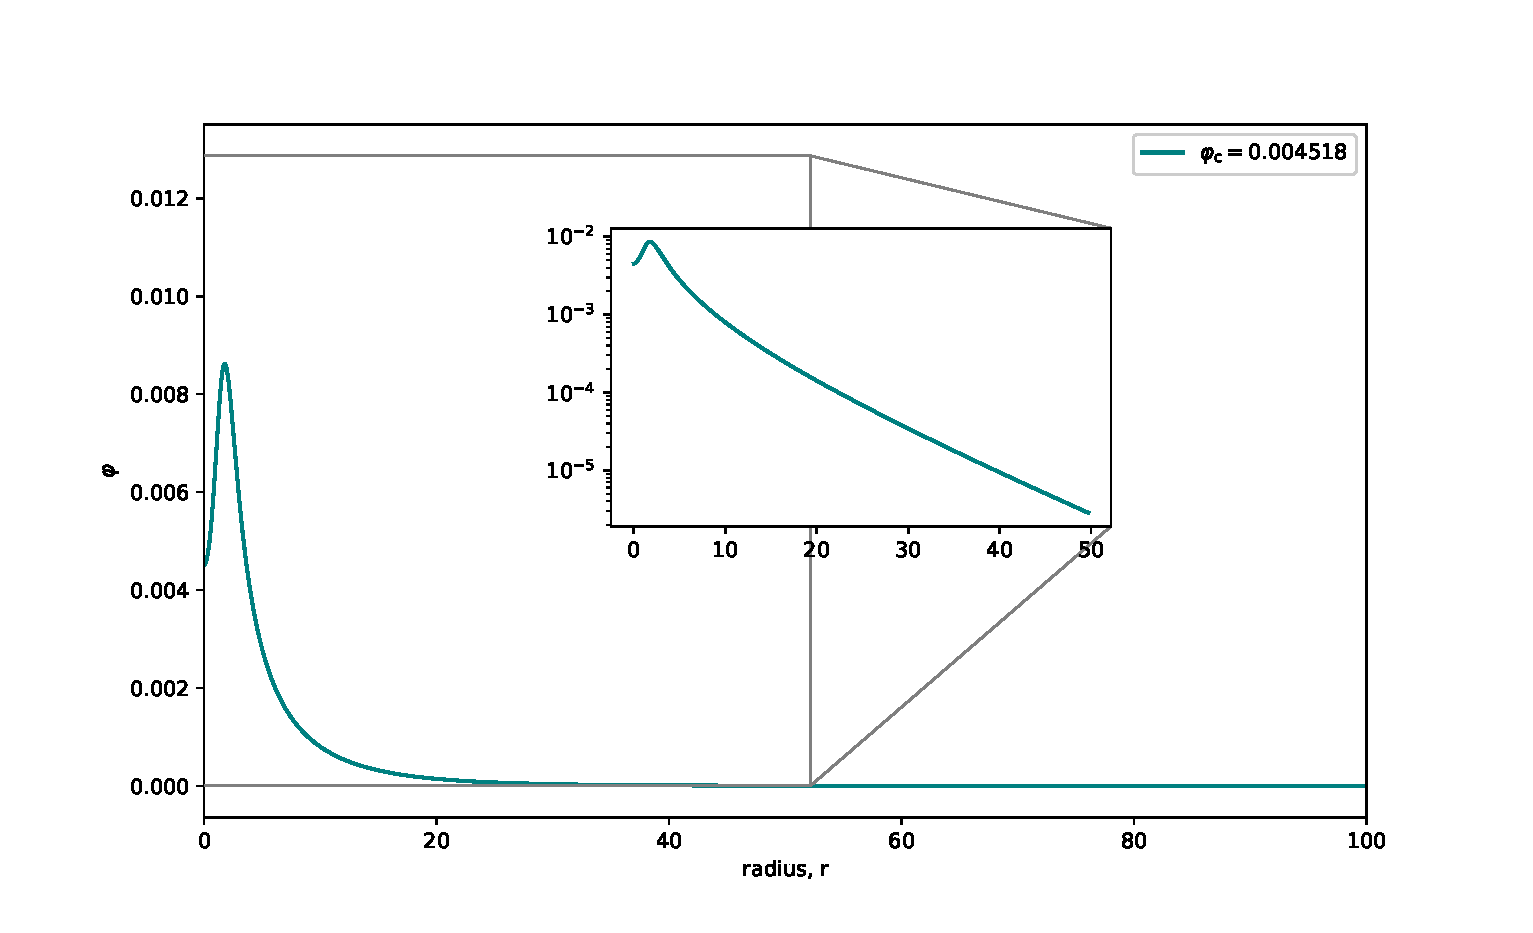
\includegraphics[width=15cm]{model-beta-12-massive.eps}
    \caption{Profile of the gravitational scalar field as a function of the radius, computed from different initial guesses for $\varphi_{\rm{c}}$ for the massive case. The threshold for satisfying \eqref{eq:criteria_massive} has been chosen empirically making sure that matching is 'smooth'. The inset includes the zoom-in onto the profile on logarithmic scale, clearly demonstrating that there are no 'kinks' in our matching procedure.}
    \label{model-beta-12-massive}
\end{figure}

%============================================================================
\newpage
\bibliographystyle{unsrt}
\bibliography{biblist}

\end{document}
